\documentclass{report}
\usepackage{graphicx} % Required for inserting images
%\usepackage{todonotes}
\usepackage{listings}
\usepackage{subcaption}
\usepackage{multicol}
\usepackage[section]{placeins}
\usepackage{amsmath}

\title{Rezepti}

\author{ Christoph Sherr , Tobias Lotz, Dominik Hummel }
\date{June 2023}

\begin{document}
\begin{figure}
    \centering
    
\includegraphics[scale=0.3]{Pictures/rezepti.png}

    \label{fig:sfig1}
\end{figure}
\maketitle

\section{Kurzbeschreibung:}
Eine Seite Für Kochrezepte von verschiedenen Ländern all around the globe.

\section{Zielgruppe Nutzer und Beeinflusser:}
Unsere Zielgruppe sind alle Personen die Kochen wollen. Nutzer könnten alle Personen sein die ein bestimmten Rezept suchen oder einfach Rezepte Endecken wollen. Beeinflusser können Firmen sein die unseren konntet für ihre Zwecke nutzen wollen zb. Influenzer die Rezepte probieren oder Firmen die Produkte durch Rezepte vermarkten wollen.

\section{Referenzdokument}
(mit Zielen, Funktionsrahmen bzw. allg. Funktionsbeschreibung, Projektrahmen, Umsetzungsstrategie, Aufgaben und Zuständigkeiten)
\newline\newline
Ziel war es ein Platform zu schaffen auf der man Rezepte mit anderen Menschen auf der ganzen Welt teilen kann oder von anderen Menschen auf der ganzen Welt Rezepte entdecken kann. 
\newline
Zu Funktionen soll gehören das man sich einen acount anlegen kann und von diBreach4-Stunner-Refuse-Doseesem aus rezepte erstellen liken und speichern kann. Es soll möglich sein rezepte ohne anmedlung einzusehen. Es soll die möglichlichleit bestehen rezepte zu suchen oder nach besrimmten zutaten ländern oder kategorien des rezeptes zu suchen. Der admin soll die funktion haben angelegte user zu löschen. 
\newline
Der Projektrahmen sind die gegebenen requirements die erfüllt wurden.
\newline
Die Umsetzungsstrategie war sehr dynamisch jeder war in einem bereich einigermaßen gut deshalb ging es einfach los und gelegentlich vergleichen bis wir an einem punkt waren das es darum ging die requirements zu erfüllen ab dann wurde mit planung schritt für schritt die requirements übernommen. 
\newline
Zuständigkeit Domme Frontend, Tobias Backend und Christoph vermittler zwischen Front und Backen und ebenfalls Entwicklung in beiden Bereichen.

\pagebreak
\section{Komplettes Product-Backlog als Tabelle}
\begin{multicols}{2}
\begin{itemize}
    \item detail view
    \item Rezept suche
    \item Startseite
    \item Rezepte aus DB laden
    \item Rating System
    \item account seite
    \item bilder hochladen
    \item rezepte erstellen
    \item admin section
    \item session management
    \item "similar" recipies section - injection resistance
    \item user profile page
    \item Filter funktion
    \item Zutaten kaufen
\end{itemize}
\end{multicols}

\pagebreak
\section{Technologien/Requirements}


\begin{itemize}
    \item Clienttechnologie: 
    \begin{itemize}
        \item CSS\\
        \item JS\\
        \item jQuery\\
        \item jQueryUI\\
        \item Bootstrap o.ä als Addon-Frameworks\\
        \item HTML5
    \end{itemize}
    
    \item Servertechnologie: 
    \begin{itemize}
        \item PHP (8.0)
        \item MariaDB (MySQL) kein PHP-Framework wie Synfony o.ä\\
        \item nginx
    \end{itemize}
    
    \item Funktionelle Vorgaben:
    \begin{itemize}
        \item Sessionverwaltung
            \begin{itemize}
                \item Wir in der common.php datei (l.7) gestartet
                \item Session expire in (l. 9 - 17)
                \item Session abfrage z.B: in admin.php (l.14-19)
            \end{itemize}
        \item Login-Logout; automatisches Logout nach bestimmter Zeit\\
            \begin{itemize}
                \item Session expire in (l. 9 - 17) 
            \end{itemize}
        \item Admin-Bereich mit Useraccount-Verwaltung\\
            \begin{itemize}
                \item In admin.php
                \item Nutzerverwaltung in den JavaScript Funktionen 
            \end{itemize}
        \item Passwort-Verwaltung\\
            \begin{itemize}
                \item In admin.php (l.105-129)
            \end{itemize}
        \item Rechte-Verwaltung (Adminrechte-Userrechte)\\
            \begin{itemize}
                \item Die Rechteverwaltung wird hier mit in Sessionvariablen gespeicherten IDs geregelt.
                z.B: in admin.php (l.14-19)
            \end{itemize}
        \item Dateneingaben client- und serverseitig prüfen (RegExp)\\
            \begin{itemize}
                \item Implementiert in common.php test\_for\_bad\_chars, test\_for\_bad\_chars\_array. Die Funktionen selbst sind in der datei common.php (l.341-345) und (l.347-353) deklariert.
            \end{itemize}
        \item Datensatzmanipulation in SQL-Server (speichern; auslesen/ausgeben; bearbeiten; löschen)\\
            \begin{itemize}
            \item Implementiert an vielen stellen im Projekt. Die Rezepte, welche auf der Startseite augegeben werden, werden aus der Datenbank geladen 
            \newline z.B: featured\_recipies (l.5-8 \dots), gespeichert in z.: admin.php (l.137-149), bearbeitet in z.B: admin.php (l.105-132), gelöscht in z.B: admin.php (l.72-99).
            \end{itemize}
        \item Konfigurationsdaten via Konfigurationsdatei einlesen\\
            \begin{itemize}
                \item Eine Konfigurationsdatei wird mit (PHP INI) realisiert. Diese wird in common.php (l.20-55) geladen und deren Daten verwendet.
            \end{itemize}
        \item Einbindung von jQuery und jQuery UI\\
            \begin{itemize}
                \item JQery und JQuery UI werden in der admin.php Datei verwendet, um z.B: einen Confirmation-Dialog zu realisieren, der den Nutzer fragt, ob eine aktion ausgefhrt werden soll, sowie auch um AJAX einzubinden.
            \end{itemize}
        \item Dynamische laden/nachladen mit Hilfe von AJAX\\
            \begin{itemize}
                \item Realisiert in admin.php (siehe oben)
            \end{itemize}
        \item Meldungsfenster und Userbestätigungen mit jQuery und jQuery UI\\
            \begin{itemize}
                \item Realisiert in admin.php (siehe oben)
            \end{itemize}
        \item Datenexport via JSON\\
            \begin{itemize}
                \item Realisiert in get\_user\_data.php
            \end{itemize}
        \item Dynamische Menüstruktur mit responsive Webdesign\\
            \begin{itemize}
                \item Auf der gesammten Seite vorhanden
            \end{itemize}
    \end{itemize}
\end{itemize}
\label{tab:my_label}

\section{Verzeichnisstruktur}
Das Projekt hat mehrere Verzeichnisse, die nur für das Setup der Dockercontainer relevant sind. Diese sind die nginx, php, site.conf und dev Verzeichnisse. Der tatsächliche code der Webapp befindet sich im Verzeichnis webdir.

\begin{figure}[!hbt]
    \centering
    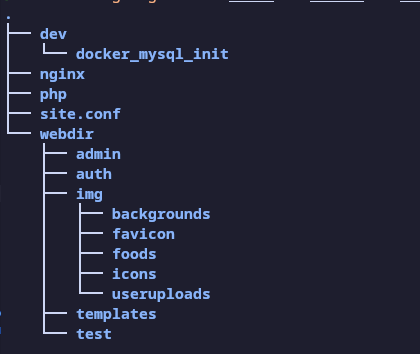
\includegraphics[scale=0.75]{Pictures/Dirs1.png}
    \caption{Directories}
    \label{fig:sfig1}
\end{figure}


\pagebreak
\section{Beschreibung der Datenstrukturen und Tabellen}

Für die Datenbank wurde nach Vorgabe MariDB verwendet. Diese Datenbank wurde in einem Dockercontainer gehostet und dann zur Bereitstellung der Daten angebunden.

\begin{figure}[!hbt]
    \centering
    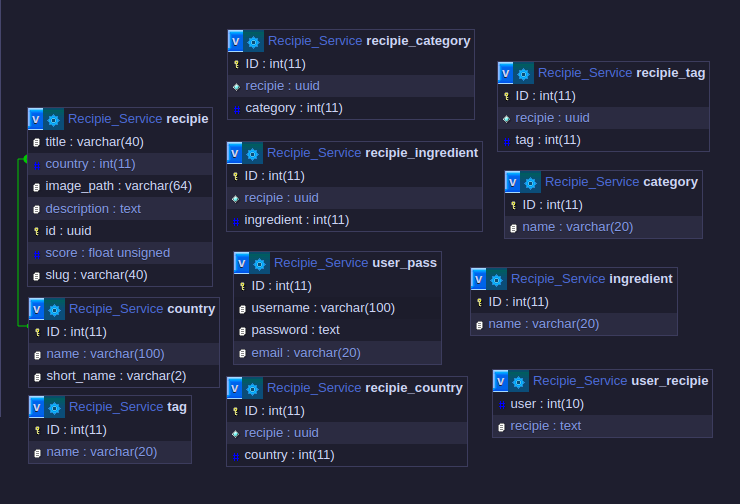
\includegraphics[scale=0.75]{Pictures/DB_Tables2.png}
    \caption{Datenbank Tabellen}
    \label{fig:sfig1}
\end{figure}




\end{document}
